\section{Study Protocol}
The data used in this study originates from an ongoing Individual Differences Project (IDP) at the Department of Anesthesia at Cincinnati Children’s Hospital and Medical Center. In this section, information on the study design will be outlined, i.e. which criteria that were set for in/exclusion, what the stimuli design was and how the data was acquired. The IDP study design involved subjecting the participant to several types of noxious stimuli. Though for the scope of this project, only the heat stimuli design will be described. 

Healthy subjects between 14 and 44 of age were recruited with no discrimination of gender and ethnicity. INFORMATION ON MEAN AGE AND STD OF THE PARTICIPANTS. As the study involved MRI scanning, subjects suffering from claustrophobia or had any electronic or metallic implants were not able to participate. Further exclusion criteria were pregnancy, skin conditions or past skin damage on or near the site of the heat stimuli delivery and intake of medications that may alter pain sensitivity or brain activation. The participants were able to withdraw from the study at any time. Additionally, the study investigators were able to withdraw participants if the they declined to comply with the experiment protocol, if a drug or pregnancy test showed positive, if there was an identification of severe brain, neurological or psychological abnormalities occurred or if the investigator assessed that it would be in the participant best interest. \\
Before enrollment in the study, the participants received a consent document (including the guardians/parents for participant under 18). First when full comprehension of the information was demonstrated the participant and guardians/parents would sign the document.

\subsubsection{Data acquisition} \label{ac}

The heat stimuli was delivered on the calf of the left leg with the Pathway stimulator\fxnote{ADD NAME AND BRAND}, while the participant was placed in a MRI scanner for recording of brain activity. For visualization of brain structures and spatial normalization of functional data high resolution T$_1$-weighted structural scans were first obtained.  MENTION WHICH EXACT SEQUENCES THAT WERE USED (MAKE A TABLE WITH THIS INFORMATION). 
Each participant went through three different heat stimuli runs with seven noxious heat stimuli in each. Each heat run had a unique sequence of 10 seconds of noxious stimuli temperatures of 47\degree C or 48\degree C interleaved with resting periods of skin temperature (35\degree C) stimuli. The design of the three heat runs can be seen in \figref{fig:meth:stimdesign}. 
Following each noxious stimulus the participant was instructed in rating the pain sensitivity and unpleasantness using a trackball/response device and a computer projected VAS, after which the participant could rest until the subsequent stimulus was delivered. The time course of each heat run followed the same pattern starting with a 20 second initiating resting period followed by seven stimulus and rating/resting periods of 2 second increasing ramp stimulus, 10 second plateau stimulus, 3 second decreasing ramp stimulus and 37-38 second rating/resting. 

\begin{figure}[H]                 
	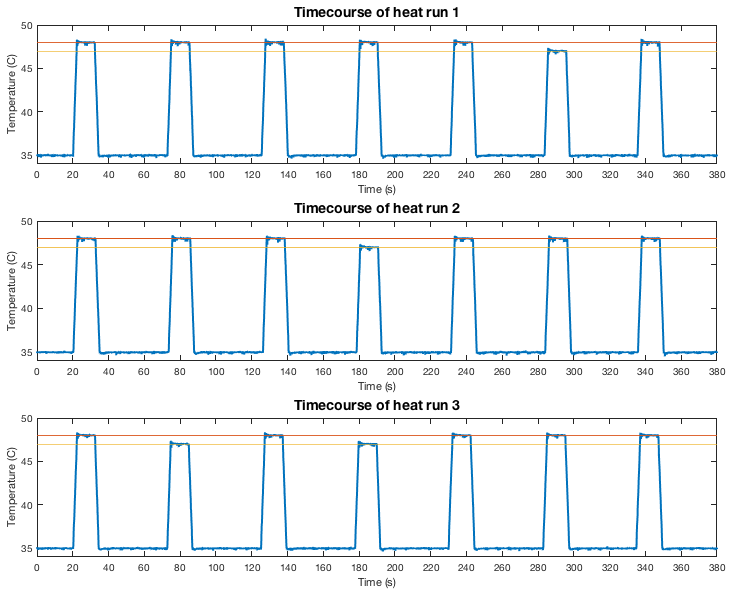
\includegraphics[width=.95\textwidth]{figures/bMethods/Stim_design} 
	 \caption{Illustrations of the time courses of heat stimuli for all three heat runs. The blue graphs depicts the temperature of the heat stimuli and the yellow and red lines are used to distinguish between 47 and 48\degree C. In the first heat run the 47\degree C stimulus was delivered during the 6th stimulus, in the second during the 4th stimulus and in the third during the 2nd and 4th stimuli. The remaining stimuli were of 48\degree C.}
	\label{fig:meth:stimdesign} 
\end{figure}



To minimize bias all participants received the same stimuli in a single-blind fashion. Furthermore, the stimuli was induced in a pseudo-random order to confine the effects of habituation and expectation. 
